\begin{figure*}[h]
    \centering
    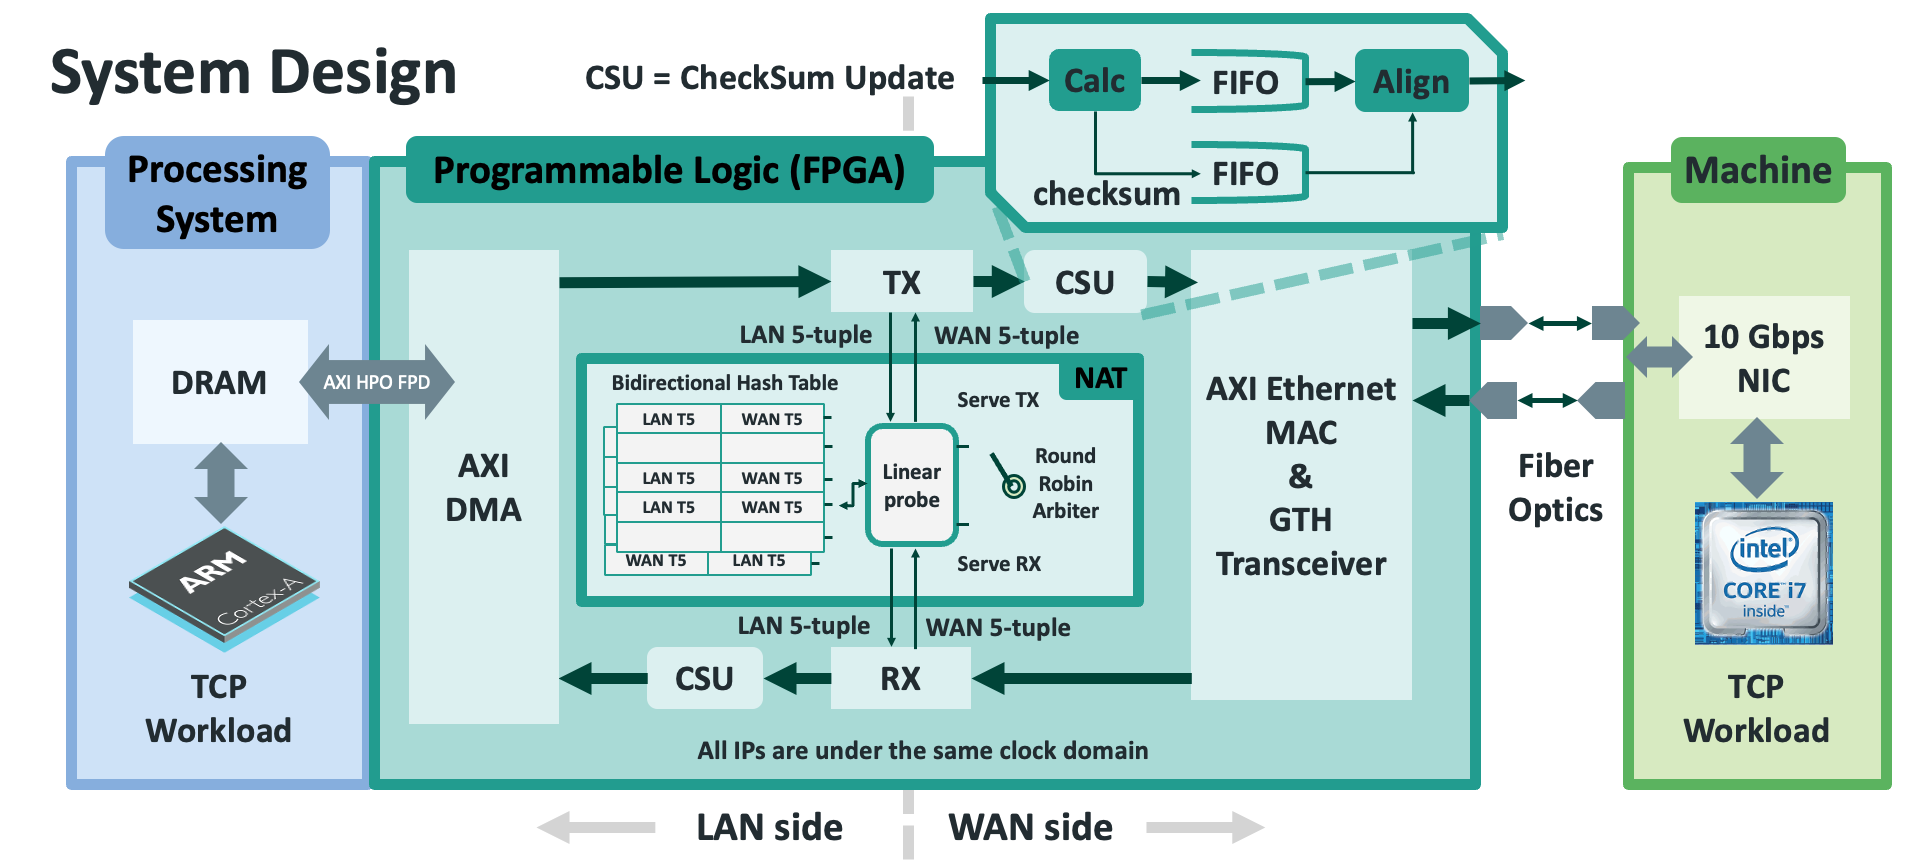
\includegraphics[width=\linewidth]{images/design.png}
    \caption{System design}
\end{figure*}
    We show our system design in this section. Our design is based on the official example of the Ethernet 10/25G system of Xilinx (referred to as the original design later). \footnote{https://github.com/Xilinx-Wiki-Projects/ZCU102-Ethernet/tree/main/2019.2/pl\_eth\_10g}

\subsection{Original Block Design}
    Before we elaborate on our design, it is necessary to show how is the original design organized as a background.

    \textbf{Components.} The design integrates PS and PL. The processing system (PS) in ZCU102 includes four ARM Cortex-A53 processors. These processors can handle general-purpose computing tasks and provide the necessary control for the entire system. The programmable logic (PL) is responsible for the custom hardware logic implementation. 
    Components like DMA, MAC, and GTH that are implemented in PL form a 10GbE network interface on the ZCU102 evaluation board. For PS, there is a Xilinx handmade Linux driver to drive this interface. We further detail the function of those components implemented in PL here:

    \begin{itemize}
    \item {DMA (Direct Memory Access)}: DMA is used for efficient data transfer between memory and peripherals without involving the processor. It enhances the throughput of data and offloads the tasks of data transfer from the processor.
    \item {MAC (Media Access Control)}: The MAC layer handles the communication protocol for the Ethernet interface. It manages frame formatting, addressing, error detection, and other protocol-related tasks.
    \item {GTH (Gigabit Transceivers)}: GTH transceivers are used for high-speed serial data communication. They facilitate the transmission and reception of data at gigabit rates.
    \end{itemize}

    \textbf{Data flow.} MAC and GTH are responsible for the transmission of data between the FPGA and the external network. Upon receiving incoming data from MAC and GTH, the DMA takes control of the data transfer process and moves it into the designated memory location. This stored data can be further processed by the processor or other components of the system.
\subsection{TX and RX}
\todo{ TX and RX are used to catch the 5-tuple, send it to NAT IP, receive response from NAT IP and replace the original 5-tuple with response. }

\subsection{NAT IP}

    Based on the original block design, we introduce a NAT (Network Address Translation) IP to intercept the communication between the MAC/GTH and DMA. Our NAT IP modifies the IP and TCP headers of the packets according to the NAT rules and maintains a bidirectional hash table to store the mappings between LAN 5 tuple and WAN 5 tuple.

    \textbf{Hash Function.} The NAT IP uses XOR operation on the 5-tuple \emph{(source IP, source port, destination IP, destination port, protocol)} as its hash function. This approach provides a quick and effective way to generate hash values for mapping.

    \textbf{Linear Probing.} To handle conflicts within the hash table, the NAT IP utilizes linear probing as a collision resolution strategy. In case of a hash collision, the algorithm linearly searches for the next available slot in the hash table until an empty slot is found.

    \textbf{Biderectional Hash Table.} Our NAT IP incorporates two hash tables. One is for the mapping from LAN 5-tuple to WAN 5-tuple, and the other maintains the reverse mapping.

    For packets from LAN to WAN, the NAT IP first computes the hash value of the LAN 5-tuple \emph{(source IP, source port, destination IP, destination port, protocol)}, and then searches for a matching entry in the hash table. If no entry is found, the NAT IP allocates a new public port from a predefined range and creates a new entry in both hash tables with the LAN 5-tuple \emph{(source IP, source port, destination IP, destination port, protocol)} and the WAN 5-tuple \emph{(public IP, public port, destination IP, destination port, protocol)}, then modifies the packet header accordingly. If a matching entry is found, the NAT IP simply replaces \emph{(source IP,  source port)} of the packet with \emph{(public IP, public port)} in the corresponding WAN 5-tuple.

    For packets from WAN to LAN, the map from WAN 5-tuple to LAN 5-tuple should exist in the normal case. Therefore, the NAT IP can modify the packet header accordingly.

    \textbf{Round Robin Arbiter.}\ It is a type of arbiter that tries to serve each requester in a circular order, ensuring that each requester can obtain resources fairly. To avoid conflicts caused by TX and RX accessing the bidirectional hash table at the same time, we use a Round Robin Arbiter in the NAT IP to control the access to the hash table. 

    We use two signals, $ready\_tx$, and $ready\_rx$, to decide which requester should be served. One ready signal is unset only in the next cycle after the end of service for the corresponding requester. In this way, a waiting requester can get served immediately after the end of service for the other. Therefore, Round Robin Arbiter achieves fair access control to the bidirectional hash table and avoids synchronization issues between TX and RX.
    
\subsection{CSU IP}
    The CSU (Checksum Update) IP is a custom IP core that recalculates the IP and TCP checksums of the packets after the NAT IP modifies the 5-tuples. It is necessary since there are sanity checks in hardware and software to validate those checksums. If mismatched, the packet will be dropped silently. 
    
    The CSU IP consists of four sub-IPs: Calc, FIFO1, FIFO2, and Align. 
    The Calc module computes the new checksum value based on the modified packet and outputs the new checksum value and the original packet to FIFO1 and FIFO2 respectively.
    The FIFO1 and FIFO2 modules are two FIFO buffers that store the new checksum value and the original packet respectively. They are used to buffer the data, waiting for the Align module to fetch. 
    The Align module is responsible for writing the new checksum value into the TCP header of the packet. It reads the data from FIFO1 and FIFO2 and locates the TCP checksum field to replace the old checksum value with the new one.


\subsection{Put It All Together}
\todo{claim: clock frequency and clock domain, how TX & RX, NAT IP, CSU IP, and DMA and MAC/GTH connect and interact with each other}